


\begin{myslide}{Slime}
  \begin{quote}
    \important{S}equentia\important{l} Funct\important{i}on Charts
    \important{M}odeling \important{E}nvironment
  \end{quote}
  \begin{itemize}
  \item \important{SFC}
    \begin{itemize}
    \item one of various  description languages for micro
      controllers
    \item international standard (IEC 61131)
    \item  Petri-net like semantics
    \item here: ``\important{poor man's SFCs}'': simplified, but with
      \important{formal} operational semantics
    \end{itemize}
  \end{itemize}
\end{myslide}

\begin{myslide}{Results}
  \begin{itemize}
  \item runnable tool, all modules integrated, executable under jdk-1.4
    \begin{itemize}
    \item graphical interface for editing
    \item checks (type checking, well-formed checking)
    \item parser
    \item simulator
    \end{itemize}
  \item \important{CD-Rom} with jar'ed tool (+ doc + sources + repos
    \ldots)
  \end{itemize}
\end{myslide}


\begin{myslide}{SFC example}
  

\vspace{-1cm}

  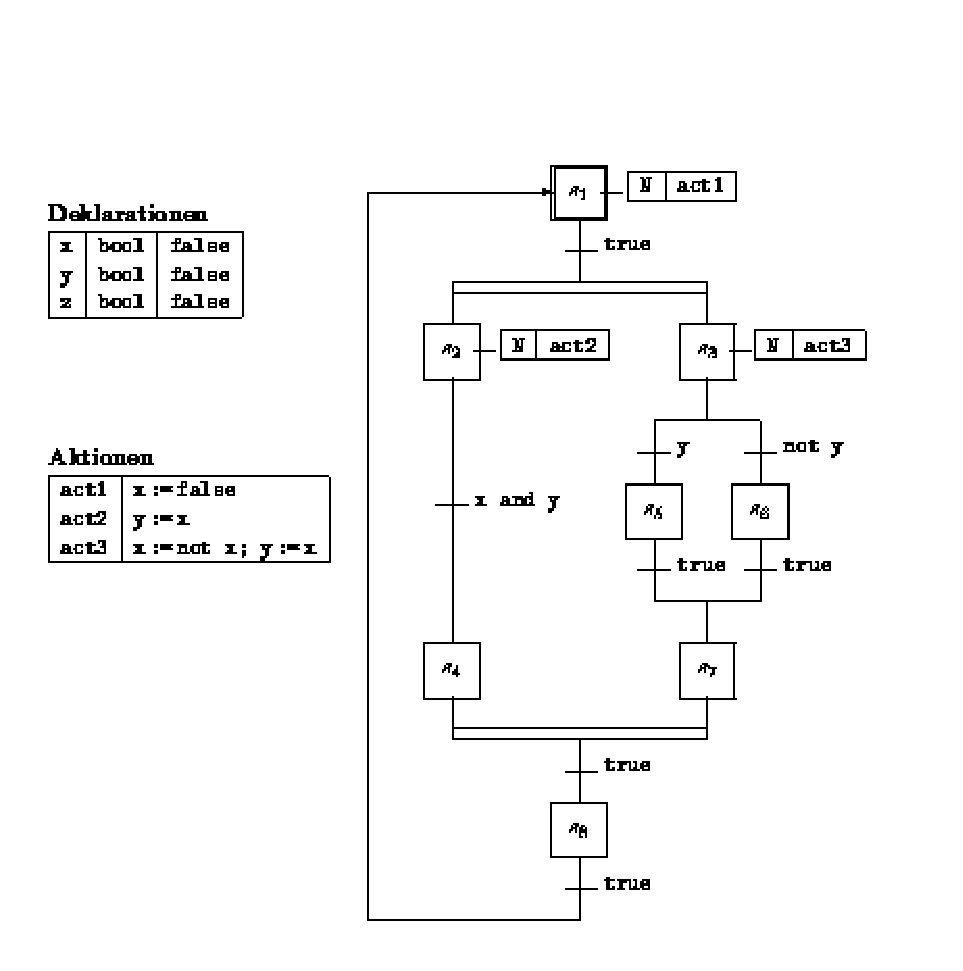
\includegraphics[height=7.5cm]{../requirements/sfc-figure}

\end{myslide}




\begin{myslide}{Develoment process}
  \begin{itemize}
  \item \important{CVS}, modules as packages
  \item Error-list, Status list
  \item email-list
  \item public \important{web-page} including \javadoc{} documentation
  \item weekly progress \important{report}
  \item 3 \important{review} meetings, including this one.
  \end{itemize}
\end{myslide}


\begin{myslide}{Timeline (planned and actual)}
  \begin{center}
   \includegraphics[height=6cm]{timeline.eps}  
    \end{center}
\end{myslide}



\begin{myslide}{Error reporting}
  \begin{lstlisting}{}
 --------------------------------------------------------
  Error <nr>:    <short description>
    package:     <in which package/class does it occur
    status:      reported|confirmed|non-confirmed|repaired
                 repaired-confirmed

               + <date> + <author>
   
    class:       fatal|non-fatal|
                 feature-request|coding convention violation ....

    description: <longer description, hints for repair>
   -----------------------------------------------------
  \end{lstlisting}
\end{myslide}



\begin{myslide}{Statistics}
  \begin{itemize}
  \item 13 official meetings
  \item 4 iterations of the requirement specification
  \item \important{> 500} emails concerning \Slime\ in my
    mailbox\footnote{including those exchanged directly with the
      participants, but without the more than 700 cvs-log emails.}
  \item approximately
    \begin{itemize}
    \item \important{100} officially reported errors\footnote{none
        confirmed \ldots}
    \item \important{170} Java files
    \item \important{200} class files, i.e. 200 public classes
    \item \important{50} \LaTeX-files (doc, web-pages, requirements)
    \item handfull of other files (Makefiles, Error lists etc.)
    \end{itemize}
  \end{itemize}
\end{myslide}





\begin{myslide}{Good}
  \begin{itemize}
  \item it's over
  \item we have a running tool ready
  \item nice result for so few people
  \item task distribution
  \item good \important{specification}: \important{formal} operational
    semantics
  \end{itemize}
  
\end{myslide}
\begin{myslide}{Neutral/beyond our control}
  \begin{itemize}
  \item not much people, 
  \item lot of (late) drop outs,\footnote{people at the beginning:
      \important{11} (except coaches), at the end: \important{4}} and
    lately announced
  \end{itemize}
\end{myslide}

\begin{myslide}{Less good}
  \begin{itemize}
  \item \important{Attracting} students
    \begin{itemize}
    \item another topic?
    \item stressing collaborative  work over programming in \Java?
    \end{itemize}
  \item \important{laaaate} first code delivery (26.\ June) /compilation,
    \important{laaate} integration (with all the consequences)
  \item we always had quite some breaches of \important{interfaces}, but:
    this year was the first time, I had to \important{discuss} why this is
    should be avoided without much discussion
  \item communication
  \item no test group, no Error ever \texttt{confirmed}
  \end{itemize}
\end{myslide}

\begin{myslide}{Next time}
  \begin{itemize}
  \item first \emph{Readme} or first \important{written plan}
    \important{required} to be \important{checked-in} in after 2 weeks
  \item stricter, enforced cvs-strategy?: \important{enforced
    compilability} for checking-in?
\item user \important{logging} (currently, I don't know how, the official
  university's server can do it, but there are other disadvantages of that
  solution)?
  \item stricter surveillance (e.g.\ for absynt), \important{watches}
  \item no \important{separation} between gui and editor? But an explicit
    \important{test} group.
  \item other means of communication? (\emph{news-group?}, cvs-logs?)
  \end{itemize}
\end{myslide}














%%%%%%%%%%%%%%%%%%%%%%%%%%%%%%%%%%%%%%%%%%%%%%%%%%%%%%%%%%%%%%%%%%%
%% $Id: content.tex,v 1.20 2002-07-19 12:43:37 swprakt Exp $
%%%%%%%%%%%%%%%%%%%%%%%%%%%%%%%%%%%%%%%%%%%%%%%%%%%%%%%%%%%%%%%%%%%
%%% Local Variables: 
%%% mode: latex
%%% TeX-master: "main"
%%% End: 
